
\documentclass[12pt]{article}

\usepackage[utf8]{inputenc}
\usepackage{amsfonts}
\usepackage{array, rotating} 
\usepackage{url}
\usepackage{hyperref}
\usepackage{amsmath}
\usepackage{fancyvrb}

\newtheorem{theorem}{Theorem} 
\newtheorem{corollary}[theorem]{Corollary} 
\newtheorem{conjecture}[theorem]{Conjecture} 
\newtheorem{lemma}[theorem]{Lemma} 
\newtheorem{proposition}[theorem]{Proposition} 
\newtheorem{definition}[theorem]{Definition} 
\newtheorem{example}[theorem]{Example} 
\newtheorem{exercise}[theorem]{Exercise} 
\newtheorem{axiom}{Axiom} 
\newtheorem{remark}{Remark} 
\def\ppp{{\mathbb{P}}}
\def\aaa{{\mathbb{A}}}
\def\fff{{\mathbb{F}}}
\def\eee{{\mathbb{E}}}
\def\qqq{\mathbb{Q}}
\def\rrr{\mathbb{R}}
\def\ccc{\mathbb{C}}
\def\zzz{\mathbb{Z}}
\def\nnn{\mathbb{N}}
\def\pf{{\bf proof}:\ }
\def\qed{$\Box$}
\def\OC{OČ}


\begin{document}

\author{David Joyner\thanks{Address: Mathematics Department
US Naval Academy, Annapolis, MD 21402, USA, wdj@usna.edu},
Ondřej Čertík\thanks{University of Nevada, Reno},
Brian E.~Granger\thanks{California Polytechnic State University, San Luis Obispo, CA}}
\title{{\small{Open Source Computer Algebra Systems}}\\ {\LARGE{SymPy}}}

\date{2011-10-31}

\maketitle

%\begin{abstract}
%In this brief survey, we look at the open-source computer
%algebra system GAP for computational group theory.
%\end{abstract}

%\vskip .5in


This survey\footnote{This paper is licensed under the
Creative Commons attribution license cc-by-sa
\url{http://creativecommons.org/licenses/by/3.0/us/},
or the Free Software Foundations GFDL
\url{http://www.fsf.org/licensing/licenses/fdl.html}
(your choice).} 
will look at SymPy, a free and open source computer algebra
system started in 2005 by the second author (\OC).
It is written entirely in Python, available from 
\url{http://sympy.org}.
SymPy is licensed under the ``modified BSD'' license, as is its
beautiful logo designed by Fredrik Johansson.

\begin{figure}[h!]
\begin{center}
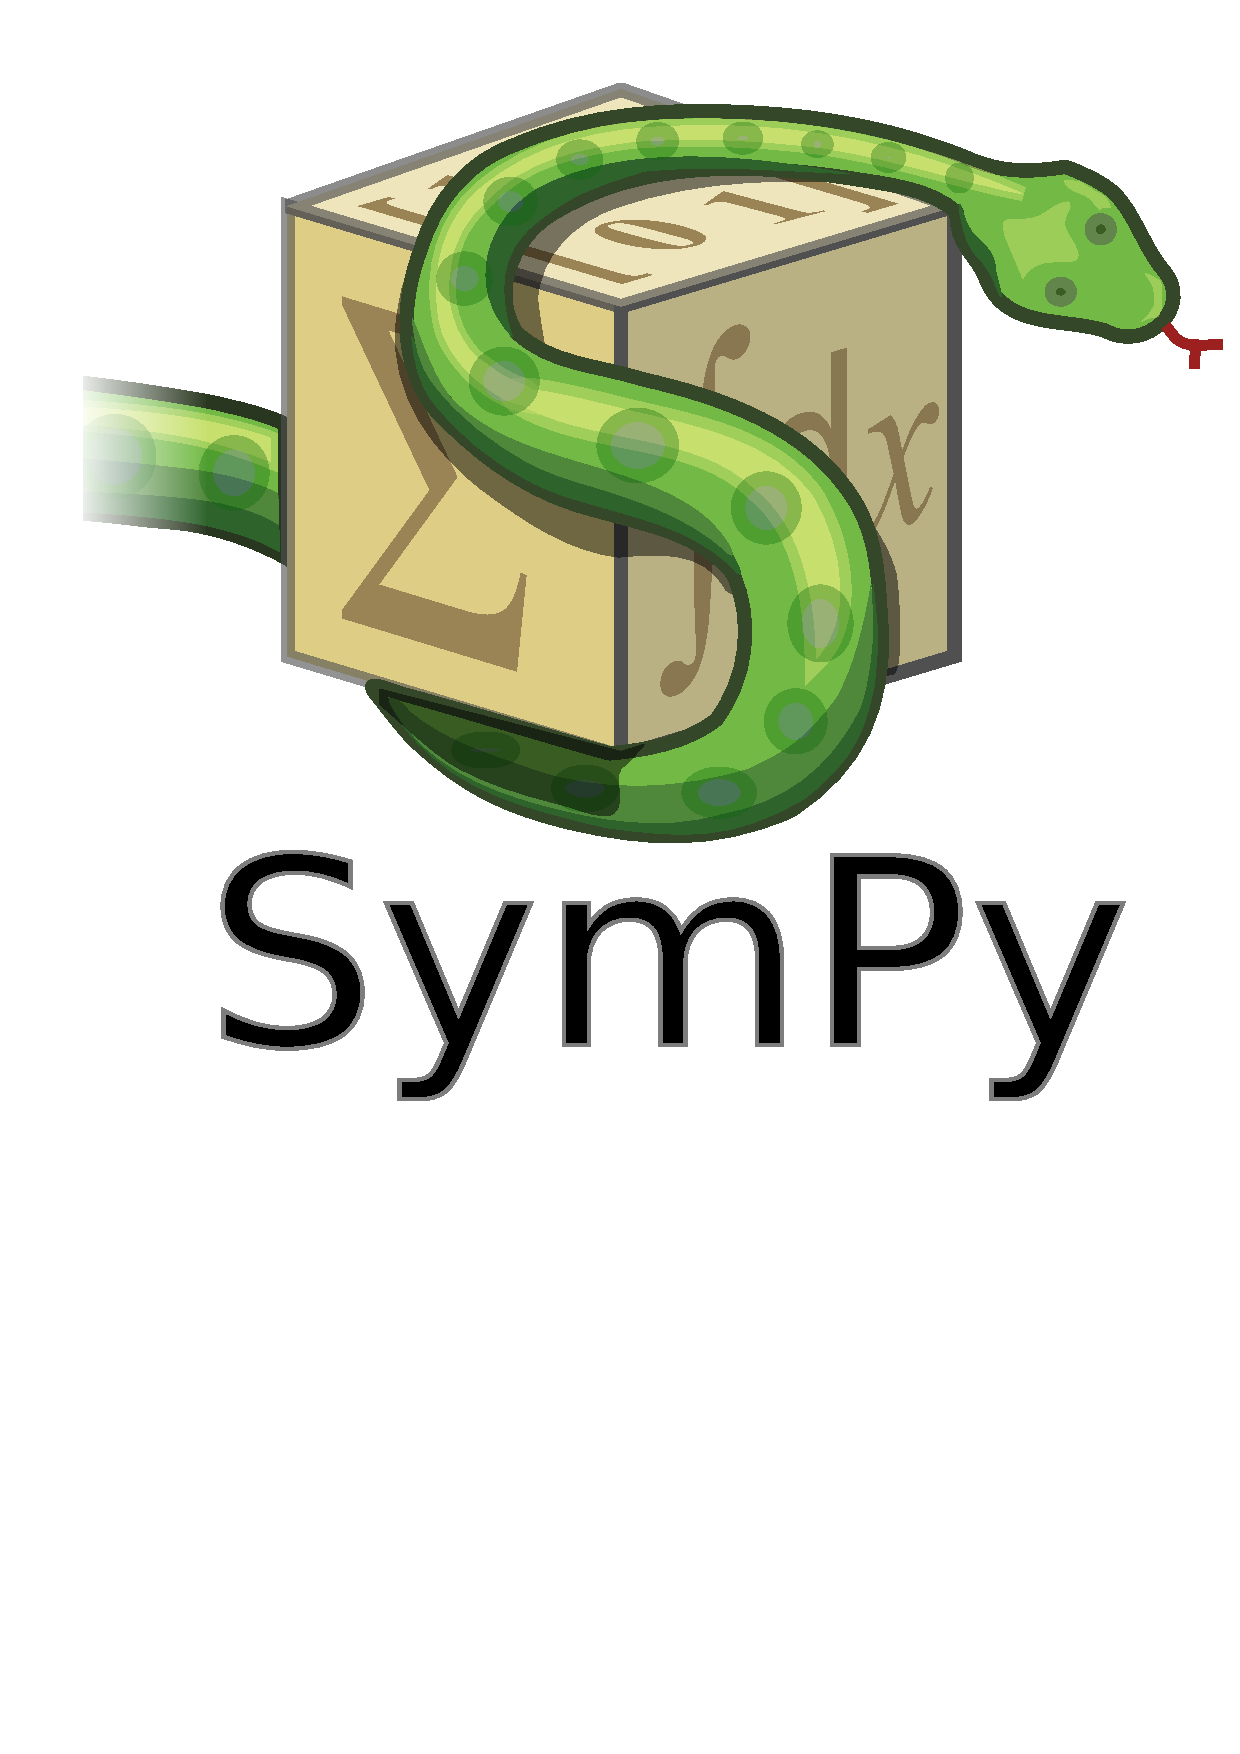
\includegraphics[height=5cm]{sympy-snake-icon.pdf}
\end{center}
\end{figure}

% There is too much white area after the image, so this reduces it:
\vskip-2cm

SymPy is also used in other mathematics software systems.
For example, SfePy (\url{http://sfepy.org/})
includes SymPy. SfePy is a software for solving systems of coupled partial differential 
equations (PDEs) by the finite element method in 2D and 3D.
The software Sage (\url{http://www.sagemath.org/}) also includes SymPy.

SymPy's latest release (as of October 2011) is 0.7.1.

\section{SymPy's history and language}

\subsection{History}

SymPy was started by \OC{} in 2005 while a
physics undergraduate at the Charles University in Prague.
He wrote initial code during the
summer, then he improved it during the summer 2006, but otherwise the project
stalled until February 2007, when
Fabian Pedregosa joined the project and helped fixed many things, contributed
documentation and made it alive again. The development hasn't stopped since
then.

Many students improved SymPy incredibly 
as part of the Google Summer of Code (GSoC):
\begin{itemize}
\item
GSoC2007: Mateusz Paprocki, Brian
Jorgensen, Jason Gedge, Robert Schwarz and Chris Wu,
\item
GSoC2008: Fredrik Johansson,

\item
GSoC2009: Priit Laes, Freddie Witherden, Aaron Meurer,
Fabian Pedregosa, Dale Peterson,

\item
GSoC2010:
Addison Cugini, Christian Muise, Aaron Meurer, Matthew Curry,
{\O}yvind Jensen,

\item
GSoC2011: Tom Bachmann, Gilbert Gede, Tomo Lazovich, Saptarshi Mandal, 
Sherjil Ozair, Vladimir Peri\'c,  Matthew Rocklin, Sean Vig, Jeremias Yehdegho.
\end{itemize}

\noindent
SymPy is a team project and it was developed by a lot of people, not
just GSoC students. For example in the early stages, Pearu Peterson
joined the development during the summer 2007 and he has made SymPy much more
competitive by rewriting the core from scratch, that has made it from 10x to
100x faster. The git repository at [1] contains all patches since July 19, 2007
and as of this writing (October 2011) it contains patches from around 141
different people (using {\tt git shortlog -ns | wc -l}).

On Jan 4, 2011 \OC{} passed the project leadership to Aaron Meurer.

\subsection{License}

SymPy uses the modified BSD license. \OC{} originally used GPL for SymPy, but
early on in 2007 switched to BSD after discussion with other developers. This
choice has worked very well for SymPy, as it doesn't enforce almost any
restrictions on how people can use SymPy (for example SymPy is included in
a commercial distribution or a paid Android application). SymPy developers
believe in allowing people to use SymPy in any way possible as well as in
creating a solid and active community around SymPy.

\subsection{Active developers}

SymPy is a project with an active community of
over 100 developers contributing to it. However, among the most active (on the
mailinglist, patches, reviews, management) as of this writing (October 2011)
are Aaron Meurer, \OC, Brian Granger, Matuesz Paprocki, Ronan Lamy, and Chris
Smith. Good (but not perfect) indicator is the number of patches contributed by
people in the last year, for example the top 10 are:

\begin{Verbatim}[fontsize=\scriptsize,fontfamily=courier,fontshape=tt,frame=single,label=git-log]

$ git shortlog -ns --since="1 year ago" | head -n 10
   590  Chris Smith
   579  Mateusz Paprocki
   413  Aaron Meurer
   172  Ronan Lamy
   149  Saptarshi Mandal
    91  Gilbert Gede
    90  Vladimir Perić
    89  Brian Granger
    79  Matthew Rocklin
    74  Ondřej Čertík
\end{Verbatim}


\subsection{Language}

\begin{quotation}
To me, there are three main
advantages of SymPy.  First, is that it is very portable,
since it is written in pure Python with no dependencies.
Second is that it is built on top of a very strong and easy to use
language, Python, which is a huge improvement over every other
computer algebra system, especially the ones that have invented their
own language.  Third, since it's just a Python module, it can very
easily be used as a library. 

{\em - Aaron Meurer}
\end{quotation}

There are even versions of SymPy for smartphones!
In addition, besides the fact that it is free, one of the best advantages 
to SymPy is how {\it easy} it is to install.
From a teacher's perspective, this is important. 

SymPy runs inside a normal Python interpreter, such as the one that
comes with your system's Python or IPython.
It is started by executing the Python script {\tt isympy}
found within SymPy's bin subdirectory.
This starts a normal Python shell (IPython shell if you have the
IPython package installed),  that (pre)executes the following commands:

\begin{Verbatim}[fontsize=\scriptsize,fontfamily=courier,fontshape=tt,frame=single,label=Python]

>>> from __future__ import division
>>> from sympy import *
>>> x, y, z, t = symbols('x y z t')
>>> k, m, n = symbols('k m n', integer=True)
>>> f, g, h = symbols('f g h', cls=Function)

\end{Verbatim}
So starting {\tt isympy} is equivalent to starting Python (or IPython)
and executing the above commands by hand. 
For example, the following simple Python commands were run 
from the command line after starting {\tt isympy}.

\begin{Verbatim}[fontsize=\scriptsize,fontfamily=courier,fontshape=tt,frame=single,label=SymPy]

>>> L = [i^2 for i in range(10) if i%2==0]
>>> L; len(L)
[2, 0, 6, 4, 10]
5

\end{Verbatim}

The following example was taken from Mateusz Paprocki's master's
degree thesis \cite{P}.

\begin{example}
{\rm
Suppose we are in possession of American coins: pennies, nickels,
dimes and quarters. We would like to compose a certain quantity out of
those coins, say 117, such that the number of coins used is
minimal. Let's forget about the minimality criterion for a moment. In
this scenario it is not a big problem to compose the requested
value. We can simply take 117 pennies and we are done, as long as we
have so many of them. Alternatively we can take 10 dimes, 3 nickels
and 2 pennies, or 2 quarters, 3 dimes, 5 nickels and 12 pennies,
etc. There are quite a few combinations that can be generated to get
the desired value. But which of those combinations leads to the
minimal number of necessary coins? To answer this question we will
take advantage of Gr\"obner bases computed with respect to a total
degree ordering of monomials.

Our problem is a minimisation problem, so we take advantage of total
degree ordering. 
This is a correct choice because total degree ordering takes monomials
with smaller sums 
of exponents first and we can observe that the smaller the sum of
exponents in a solution 
to our coins problem will be, the less coins will be needed. So, the
chosen ordering of 
monomials encodes the cost function of our problem.

How to get the minimal number of required coins? Suppose we take any
admissible solution 
to the studied problem. This can be the trivial solution in which we
take 117 pennies or any 
other such that the total value of coins is equal to 117. We encode
the chosen solution as a 
binomial with numbers of particular coins as exponents of $p, n, d$ and
$q$, and we reduce this 
binomial with respect to the Gr\"obner basis G utilizing
graded lexicographic ordering of monomials.


\begin{Verbatim}[fontsize=\scriptsize,fontfamily=courier,fontshape=tt,frame=single,label=SymPy]

>>> var('p, n, d, q')
(p, n, d, q)
>>> F = [p**5 - n, p**10 - d, p**25 - q]
>>> G = groebner(F, order='grlex')
>>> reduced(p**117, G, order='grlex')[1]
     2  4
d n p  q

\end{Verbatim}

\noindent
The answer, that we were able to compute with SymPy, is 1 dime, 1 nickel,
2 pennies, and 4 quarters which altogether give the requested value of 117.
This is also the minimal solution to our problem.

This example showed SymPy's ability to compute with Gr\"obner basis, but the
problem can be solved without such advanced machinery using greedy approach
that involves only basic arithmetics:

\begin{Verbatim}[fontsize=\scriptsize,fontfamily=courier,fontshape=tt,frame=single,label=SymPy]

>>> k = Symbol('k', integer=True)
>>> coin_values = zip(var("p, n, d, q"), [1, 5, 10, 25])
>>> total, coin_counts = 117, []
>>> for coin, value in reversed(coin_values):
...     count = floor(solve(k*value <= total, k).rhs)
...     coin_counts.append((coin, count))
...     total -= count*value
...
>>> Mul(*[ coin**count for coin, count in coin_counts ])
     2  4
d n p  q

\end{Verbatim}

}
\end{example}




\section{Documentation and capabilities}



\subsection{Basics}

A great deal of information about SymPy is available on its website. 


\begin{itemize}
\item
Internet:
\newline
{\it Website} :
\newline
\url{http://sympy.org/}


\item
Documentation:
\newline
{\it On-line reference manual}: 
\newline
\url{http://docs.sympy.org/}
\newline
\url{http://docs.sympy.org/0.7.1/tutorial.html}
\newline
\url{https://github.com/sympy/sympy/wiki}
%\newline
%{\it Bibliography}: 

\item
{\it Talks, blogs, papers, and lecture notes}:
\newline
\url{http://planet.sympy.org/}
\newline
\url{https://github.com/sympy/sympy/wiki/SymPy-Papers}

\item
Interfaces:
\newline
{\it Command line}
\newline
There are very useful command-line history, tab-completion, and
command-line help features available.
\newline
{\it Online version}:
\newline
\url{http://live.sympy.org/}
\newline
The Sage notebook interface (available in any Sage installation,
available from \url{http://www.sagemath.org/}, or on-line at:
\url{http://www.sagenb.org/} (select {\tt sympy} in the drop-down menu).
\item
Availability:
\newline
{\it Source code and binaries}:
\url{http://sympy.org/download.html}

SymPy is easy to install on all operating systems that 
support Python (e.g., MS Windows, Mac OSs, All flavors of Linux, and
so on).

There is also a version for the iPhone which is available separately
from the iTunes online store (look for ``Python Math'' or
go to \url{http://sabonrai.com/wp/pythonmath/}).

For the smartphone OS ``Maemo'', there is a Sympy app described at
\url{http://www.robertocolistete.net/Integral/}.


\item
{\it Support}:
\newline
There is an email list for SymPy support and development:
\newline
\url{http://groups.google.com/group/sympy?pli=1}
\newline
{\tt sympy@googlegroups.com}


\item
{\it License}:
\newline
Modified BSD. 

\end{itemize}



\subsection{Capabilities}

Currently, SymPy core has extensive computational capabilities including:

\begin{itemize}
\item
    basic arithmetics $*,/,+,-,**$,
\item
    basic simplification (like $a*b*b + 2*b*a*b \mapsto 3*a*b^2$),
\item
    expansion (like $(a+b)^2 \mapsto a^2 + 2*a*b + b^2$),
\item
    functions ($\exp, \ln$, \dots),
\item
    complex numbers (like $\exp$(I*x).expand(complex=True) $\mapsto$
    $\cos(x)+I*\sin(x)$),
\item
    differentiation,
\item
    taylor (laurent) series,
\item
    substitution (like $x \mapsto \ln(x)$, or $\sin \mapsto \cos$),
\item
    arbitrary precision integers, rationals and floats,
\item
    noncommutative symbols,
\item
    pattern matching .
\end{itemize}
Then there are many SymPy modules, such as (for example) for these tasks:
\begin{itemize}
\item
    more functions ($\sin, \cos, \tan$, atan, asin, acos, factorial, zeta, legendre),
\item
    limits (like limit($x*\log(x), x, 0) \to 0$),
\item
    integration using extended Risch-Norman heuristic,
\item
    polynomials (division, gcd, square free decomposition, groebner bases, factorization),
\item
    solvers (algebraic, difference and differential equations, and systems of equations),
\item
    symbolic matrices (determinants, LU decomposition...),
\item
  Pauli and Dirac algebra,
\item
    geometry module,
\item
    plotting (2D and 3D) .
\end{itemize}

\subsubsection{Quantum physics}

Thanks mostly to work done by B.G., and students he has directed, SymPy
has extensive capabilities in quantum physics.  These capabilities are focused
on the various symbolic manipulations that arise in quantum mechanics,
rather than on more traditional numerical computations.

To enable these symbolic manipulations to be performed using SymPy, we have
implemented the Dirac notation in its most abstract and general form. This includes
all of the needed mathematical entities: Hilbert spaces, bras and kets, operators,
inner/outer/tensor products, commutators, anticommutators and so on.

The object-oriented nature of SymPy/Python has been particularly valuable in
this work.  The various mathematical entities listed above are implemented
as base classes and then specific physical systems are implemented through
subclassing.  Thus, for example, when a spin operator is defined, it immediately
inherits all of the capabilities of general hermitian operators.  This allows new physical
systems to be implemented quickly and easily.

The following quantum mechanical system have been implemented in this manner:
i) quantum angular momentum including spin coupling, ii) second quantization for
fermions and bosons, iii) gates and qubits used in quantum computing and quantum
information, iii) position and momentum eigenstates and a variety of systems that
utilize them and iv) density operators and matrices for representing mixed states.

The classes we have created for quantum computing are now being used
in a research context. Being able to handle gates and qubits symbolically
is extremely important, as the alternative requires constructing and multiplying
extremely large matrices. This is enabling B.G. and co-workers to develop new
optimization approaches for quantum circuits and algorithms.

As an example of the quantum computing capabilities in SymPy, we show how to
apply a Hadamard gate to a qubit symbolically:

\begin{Verbatim}[fontsize=\scriptsize,fontfamily=courier,fontshape=tt,frame=single,label=SymPy]

>>> from sympy.physics.quantum import qapply
>>> from sympy.physics.quantum.gate import H
>>> from sympy.physics.quantum.qubit import Qubit
>>> c = H(0)*Qubit('0')
>>> qapply(c)
sqrt(2)*|0>/2 + sqrt(2)*|1>/2

\end{Verbatim}

In this example, we illustrate the rewriting of two angular momentum states in different
bases and show the integrated latex rendering of SymPy:

\begin{Verbatim}[fontsize=\scriptsize,fontfamily=courier,fontshape=tt,frame=single,label=SymPy]

>>> from sympy import S, latex
>>> from sympy.physics.quantum.spin import JxKet
>>> latex(JxKet(S(1)/2,S(1)/2).rewrite('Jz'))
\frac{1}{2} \sqrt{2} {\left|\frac{1}{2},- \frac{1}{2}\right\rangle } + \frac{1
}{2} \sqrt{2} {\left|\frac{1}{2},\frac{1}{2}\right\rangle }
>>> latex(JxKet(1,1).rewrite('Jz'))
\frac{1}{2} {\left|1,-1\right\rangle } + \frac{1}{2} \sqrt{2} {\left|1,0\right
\rangle } + \frac{1}{2} {\left|1,1\right\rangle }

\end{Verbatim}
This will print:

\[
\frac{1}{2} \sqrt{2} {\left|\frac{1}{2},- \frac{1}{2}\right\rangle } + \frac{1
}{2} \sqrt{2} {\left|\frac{1}{2},\frac{1}{2}\right\rangle }
\]

\[
\frac{1}{2} {\left|1,-1\right\rangle } + \frac{1}{2} \sqrt{2} {\left|1,0\right
\rangle } + \frac{1}{2} {\left|1,1\right\rangle }
\]

For further details, see the papers by Cugini \cite{Cug}
and Curry \cite{Cur}, or blog posts related to quantum mechanics on 
Planet SymPy (\url{http://planet.sympy.org/}).

\subsubsection{Packages}

To plot a function in SymPy you need to install a separate plotting
package, such as matplotlib or pyglet.
To install them into your local Python install, follow the
instructions on their website (that is,
\url{http://www.pyglet.org/} or
\url{http://matplotlib.sourceforge.net/}).

\subsubsection{Examples}

This section merely presents a few examples to illustrate some of 
SymPy's functionality.

To plot a function in 2d, such as $y=\sin(x)$,
use the following SymPy commands.

\begin{Verbatim}[fontsize=\scriptsize,fontfamily=courier,fontshape=tt,frame=single,label=SymPy]

>>> x = Symbol("x")
>>> Plot(sin(x), [x, -3, 3])
[0]: sin(x), 'mode=cartesian'

\end{Verbatim}

\noindent
A separate window will pop-up with your (color) plot in it.
See Figure \ref{fig:sympy-plots}.

To plot a surface in 3d, such as $z=xy^3-yx^3$,
use the following SymPy commands.

\begin{Verbatim}[fontsize=\scriptsize,fontfamily=courier,fontshape=tt,frame=single,label=SymPy]

>>> var('x y z')
>>> Plot(x*y**3-y*x**3)

\end{Verbatim}

\noindent
A separate window will pop-up with your (color) plot in it.
See Figure \ref{fig:sympy-plots}.


\begin{figure}[h!]
\begin{minipage}{\textwidth}
\begin{center}
%\vspace{8.0 cm}
\begin{tabular}{cc}
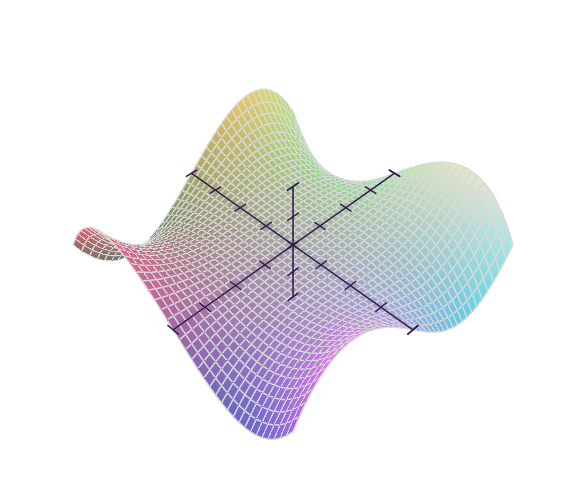
\includegraphics[height=5cm,width=5cm]{oscas-sympy-plot1b}
 &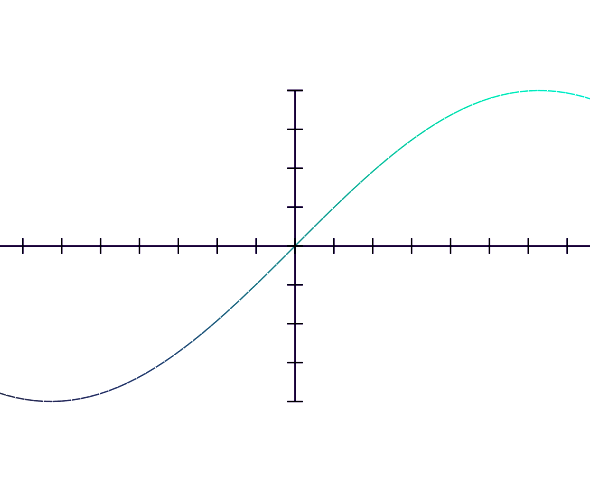
\includegraphics[height=5cm,width=5cm]{oscas-sympy-plot2b} \\
\end{tabular}
\end{center}
\end{minipage}
\caption{2D and 3D plots using SymPy}
\label{fig:sympy-plots}
\end{figure}

SymPy has good functionality with linear algebra.
The method {\tt rref} returns the row-reduced echelon form of a matrix,
as well as a list of the pivot columns.

\begin{Verbatim}[fontsize=\scriptsize,fontfamily=courier,fontshape=tt,frame=single,label=SymPy]

>>> M = Matrix(3,3,lambda i,j: i+j)
>>> print M
[0, 1, 2]
[1, 2, 3]
[2, 3, 4]
>>> print M.rref()
([1, 0, -1]
[0, 1,  2]
[0, 0,  0], [0, 1])

\end{Verbatim}

\noindent
Indeed, there is a pivot in the first two columns but not the
third, so SymPy returns only $[0,1]$, as it should.

\begin{Verbatim}[fontsize=\scriptsize,fontfamily=courier,fontshape=tt,frame=single,label=SymPy]

>>> M = Matrix([[1,1,2],[1,2,1],[2,1,1]])
>>> print M
[1, 1, 2]
[1, 2, 1]
[2, 1, 1]
>>> print M.eigenvals()
{1: 1, -1: 1, 4: 1}
>>> print M.eigenvects()
[(1, 1, [[ 1]
[-2]
[ 1]]), (-1, 1, [[-1]
[ 0]
[ 1]]), (4, 1, [[1]
[1]
[1]])]
>>> print M.charpoly(x)
Poly(x**3 - 4*x**2 - x + 4, x, domain='ZZ')

>>> lam = M.eigenvals()
>>> lam.keys()                
[1, -1, 4]
>>> lamb = lam.keys()
>>> expand((x-lamb[0])*(x-lamb[1])*(x-lamb[2]))
 3      2        
x  - 4*x  - x + 4

\end{Verbatim}

\noindent
In the last command, we merely verify that the characteristic
polynomial is indeed a polynomial whose roots are the eigenvalues.

Thanks mostly to the work of Aaron Meurer, 
SymPy can solve higher order linear ordinary differential equations.
See Meuer \cite{M} for details of the implementation.
To solve the $3$-rd order constant coefficient ordinary differential
equation,

\[
y'''-3y''+3y'-y=10e^x,
\]
use the following SymPy commands.

\begin{Verbatim}[fontsize=\scriptsize,fontfamily=courier,fontshape=tt,frame=single,label=SymPy]

>>> x = Symbol("x")
>>> y = Function('y')
>>> de = y(x).diff(x,3)-3*y(x).diff(x,2)+3*y(x).diff(x)-y(x)-6*exp(x)
>>> soln = dsolve(de, y(x))
>>> print soln
y(x) == (C1 + C2*x + C3*x**2 + x**3)*exp(x)

\end{Verbatim}

\noindent
Surprisingly, it seems Maxima cannot do this at the present time.

SymPy handles easily a wide range of calculus computations, as the following 
commands illustrate.

\begin{Verbatim}[fontsize=\scriptsize,fontfamily=courier,fontshape=tt,frame=single,label=SymPy]

>>> print legendre(8, x).diff(x)
6435*x**7/16 - 9009*x**5/16 + 3465*x**3/16 - 315*x/16
>>> print integrate(legendre(8, x),x)
715*x**9/128 - 429*x**7/32 + 693*x**5/64 - 105*x**3/32 + 35*x/128
>>> j0 = lambda x: besselj(0,x)
>>> limit(j0(x),x,0)
besselj(0, 0)
>>> N(limit(j0(x),x,0))
1.00000000000000

\end{Verbatim}

SymPy handles Taylor series expansions with no problem.

\begin{Verbatim}[fontsize=\scriptsize,fontfamily=courier,fontshape=tt,frame=single,label=SymPy]

>>> x = Symbol('x')
>>> f = 1/cos(x)
>>> print f.series(x, 0, 10)
1 + x**2/2 + 5*x**4/24 + 61*x**6/720 + 277*x**8/8064 + O(x**10)

\end{Verbatim}

Did you know SymPy can solve a linear recurrence sequence?
For example, consider

\[
 u_{n+2} = 2  u_{n+1} + 8  u_{n}, 
\]
where we know $u_{0} = 2$ and $u_{1} = 7$.

\begin{Verbatim}[fontsize=\scriptsize,fontfamily=courier,fontshape=tt,frame=single,label=SymPy]

>>> n = Symbol('n', integer=True)
>>> u = Function('u')
>>> f=u(n+2)-2*u(n+1)-8*u(n)
>>> print rsolve(f, u(n), {u(0):2, u(1):7})
(-2)**n/6 + 11*4**n/6

\end{Verbatim}

SymPy contains wide range of special functions and it can easily be used to
evaluate complicated expressions. For example here is how to evaluate the
formula for the third order perturbative correction to the
magnetic moment of an electron in quantum electrodynamics (this example also
shows how to sum an infinite series), you can compare the formula and the value
with the abstract of the paper \cite{QED} and see that it agrees:

\begin{Verbatim}[fontsize=\scriptsize,fontfamily=courier,fontshape=tt,frame=single,label=SymPy]

>>> from sympy import pi, zeta, S, log, summation, var, oo
>>> var("n")
n
>>> a4 = summation(1/(2**n * n**4), (n, 1, oo))
>>> A_3 = 83*pi**2*zeta(3)/72 - 215*zeta(5)/24 + 100*(a4 + log(2)**4/24 - \
...         pi**2*log(2)**2/24)/3 - \
...         239*pi**4/2160 + 139*zeta(3)/18 - 298 * pi**2 * log(2)/9 + \
...         17101 * pi**2 / 810 + S(28259)/5184
>>> A_3.n()
1.18124145658720

\end{Verbatim}

\vskip 0.3in

In short, if you need to use a free mathematics program in teaching or
research, and one which is easily installed on various platforms,
SymPy is a great place to start. If you get stuck, there is plenty of
information
on-line, or you can join the SymPy googlegroups and
email your question to {\tt sympy@googlegroups.com}.

\vskip 0.3in

\noindent
{\it Acknowledgements}:
We thank Aaron Meurer, Mateusz Paprocki and Vladimir Peri\'c
for helpful comments and corrections. (Any remaining errors are of course our
responsibility). Some of the material above is taken 
with only slight modification from Paprocki's paper
\cite{P}, the tutorial \cite{PM}, or the documentation at the official SymPy website
\cite{S}.



\begin{thebibliography}{99}

\bibitem[Cug]{Cug}
Addison Cugini,
{\it Quantum Mechanics, Quantum Computation, and the Density Operator in SymPy},
California Polytechnic State University, Senior Thesis, 2011.
\newline
\url{http://digitalcommons.calpoly.edu/physsp/38}

\bibitem[Cur]{Cur}
Matthew Curry,
{\it Symbolic Quantum Circuit Simpliflcation in SymPy},
California Polytechnic State University, Senior Thesis, 2011.
\newline
\url{http://digitalcommons.calpoly.edu/physsp/39}

\bibitem[M]{M} A. Meurer, 
{\it Variation of Parameters and More}, blog post available at
\newline
\url{http://asmeurersympy.wordpress.com/2009/08/01/variation-of-parameters-and-more/}.

\bibitem[P]{P}  
Mateusz Paprocki,
{\it  Design and Implementation Issues of a Computer Algebra System 
in an Interpreted, Dynamically Typed Programming Language},
Master's Thesis, 2010, University of Technology of
Wroclaw,  Poland.
\newline
\url{https://github.com/mattpap/masters-thesis}
\newline
\url{http://mattpap.github.com/masters-thesis/html/index.html}

\bibitem[PM]{PM}  
------ and Aaron Meurer,
{\it Guide to symbolic mathematics with SymPy},
SciPy conference 2011 presentation, 
\newline
\url{http://mattpap.github.com/scipy-2011-tutorial/html/mathematics.html}

\bibitem[QED]{QED}
S.Laporta, E.Remiddi
{\it The analytical value of the electron (g-2) at order $\alpha^3$ in QED},
Phys.Lett. B379 (1996) 283-291
\newline
\url{http://arxiv.org/abs/hep-ph/9602417}


\bibitem[S]{S}  SymPy website
\newline
\url{http://www.sympy.org/}



\end{thebibliography}


\end{document}


+++++++++++++++++++++

\bibitem[V]{V}
Sean Vig's 2011 GSoC Project blog,
Developing Wigner-3nj Symbols in SymPy
http://seanvig.blogspot.com/



\bibitem[L]{L}
Tomo Lazovich's SymPy Blog
\newline
\url{http://lazovichsympy.wordpress.com/}
